\documentclass[10pt,a4paper]{article}
\usepackage[utf8]{inputenc}
\usepackage{amsmath}
\usepackage{amsfonts}
\usepackage{amssymb}
\usepackage{graphicx}
\usepackage{a4wide}
\usepackage{pgfplots}
\usepackage{hyperref}
\usepackage{parskip}
\begin{document}
	\section*{Kriterien für die Lesbarkeitsanalyse}
	\subsection*{Wortlänge}
	Hierfür wird zunächst die durchschnittliche Wortlänge analysiert und normiert. 
	Sei $ W $ die Menge aller Wörter $ w_i $ im zu analysierenden Text mit Wortlänge $wl_i= |w_i| $. Die minimale Wortlänge ist 1 (bzw. 2 im Deutschen), die maximale ist $ l_{max}=max(|w_i|) $ bzgl. aller Wörter $ w_i\in W $. 
	
	Der Lesbarkeitswert jedes Wortes wird normiert durch $ \frac{|w_i|}{l_{max}}$ und der summierte Wert des entsprechenden (Ab-)satzes durch die Anzahl der Wörter $ |W| $ geteilt. Anschließend wird der Wert z.B. auf Farbwerte zwischen blau $ (32,62,181) $, weiß und rot $ (186,57,44) $ abgetragen.\\

		\pgfplotsset{compat=1.10}
		\begin{figure}[!h]
			\centering
			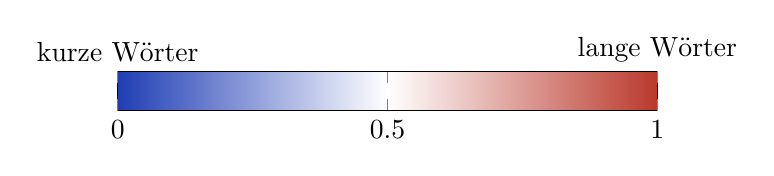
\begin{tikzpicture}
			\begin{axis}[
			colormap={lolmap}{[1cm] 
				rgb255(0cm)=(32,62,181) color(5cm)=(white) rgb255(10cm)=(186,57,44)}, colorbar horizontal, colorbar/width=.5cm, 
				colorbar style={xtick={0,.5,1},
				xlabel near ticks, 
				extra x ticks={0,1},
				extra x tick labels={kurze Wörter, lange Wörter}, 
				extra x tick style={ticklabel pos=right}   
				},
				hide axis
			]
			%\addplot[mesh, point meta=y, line width=4mm, samples=150] {x^2}; % Some graph to show...
			\end{axis}
			\end{tikzpicture}
		\end{figure}
	\subsection*{Komplexität der Vokabeln}
	Hier wird der Prozentanteil eines Absatzes/Satzes gemessen, der nicht in einer Liste häufig verwendeter Wörter vorkommt. Dazu kann entweder Wikipedia\footnote{\url{https://en.wiktionary.org/wiki/Wiktionary:Frequency_lists\#German}} (deutsch/englisch), ein Korpus aus Zeitungsartikeln\footnote{\url{http://wortschatz.uni-leipzig.de/html/wliste.html}} oder evtl. eine fachspezifische Textsammlung ausgewertet werden. Der Anteil der Wörter $ w_i $, die nicht in der Liste $ L $ sind, wird dann durch die Anzahl $ |W| $ der Wörter im zu analysierenden Text $ W $ geteilt, also $  \text{Komplexität}_W= \frac{|w_i\not\in L|}{|W|}$ in Prozent.\\

		\begin{figure}[!h]
			\centering
			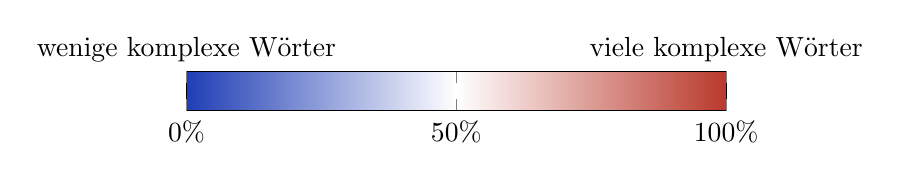
\begin{tikzpicture}
			\begin{axis}[
			colormap={lolmap}{[1cm] 
				rgb255(0cm)=(32,62,181) color(5cm)=(white) rgb255(10cm)=(186,57,44)}, colorbar horizontal, colorbar/width=.5cm, 
			colorbar style={xtick={0,.5,1},
				xticklabels={0\%,50\%,100\%},
				xlabel near ticks, 
				extra x ticks={0,1},
				extra x tick labels={wenige komplexe Wörter, viele komplexe Wörter}, 
				extra x tick style={ticklabel pos=right}   
			},
			hide axis
			]
			%\addplot[mesh, point meta=y, line width=4mm, samples=150] {x^2}; % Some graph to show...
			\end{axis}
			\end{tikzpicture}
		\end{figure}
	\subsection*{Nominalisierungen}
	\subsection*{Satzlänge}
	\subsection*{Komplexität der Satzstruktur}
\end{document}